% "spell_check": true,
% "dictionary": "Packages/Language - English/en_US.dic"
\documentclass[preprint,aps,prb,floatfix]{revtex4-1}
%\documentclass[journal=jpcbfk, manuscript=article]{achemso}
%\usepackage{achemso}
%\setkeys{acs}{usetitle = true}
\usepackage[pdftex]{graphicx,color,epsfig}
\usepackage{xcolor}
\usepackage{graphicx}
\usepackage{amsfonts}
\usepackage{amssymb}
\usepackage{bm} % Bold math
\usepackage[figuresleft]{rotating}
\usepackage[mathscr]{eucal}
\usepackage{threeparttable}
\usepackage{amsmath}
\usepackage[sort&compress]{natbib}
\usepackage{multirow}
\usepackage{booktabs}
\usepackage{geometry}
\usepackage{mathtools} % Boxes
\usepackage{siunitx} % SI units
\usepackage{enumitem} % Resetting counter
\usepackage{braket}
\usepackage{float}
\usepackage{threeparttable}
\usepackage{gensymb}
\usepackage{ragged2e}
\usepackage{setspace}
\usepackage{cleveref}
\usepackage{wrapfig}
\usepackage[utf8]{inputenc} % Required for inputting international characters
\usepackage[T1]{fontenc} % Output font encoding for international characters
\usepackage{mathpazo} % Palatino font
\usepackage{chngpage}
\usepackage{subfig} % http://ctan.org/pkg/subfig
\usepackage{xr} % external references

\maxdeadcycles=200 % required to fix low level error

% Folder for figures
\newcommand{\figfile}{C:/Users/Hayden/Documents/Patey_Lab/ThesisCodeBase/Manuscript_1.0/figures}
\newcommand{\HOS}{{\color{red}HOS}}
\newcommand{\Ham}{\widehat{\mathcal{H}}}
\externaldocument{DFT_Lithium_Halides_Supplementary_Info}

% End of Section Numbering Customization

\AtBeginDocument{
\heavyrulewidth=.08em
\lightrulewidth=.05em
\cmidrulewidth=.03em
\belowrulesep=.65ex
\belowbottomsep=0pt
\aboverulesep=.4ex
\abovetopsep=0pt
\cmidrulesep=\doublerulesep
\cmidrulekern=.5em
\defaultaddspace=.5em
}


\date{\today}

\begin{document}
%\bibliographystyle{aip}
\bibliographystyle{achemso}

\author{H. Scheiber}
\email{scheiber@chem.ubc.ca}
\author{G. N. Patey}
\email{patey@chem.ubc.ca}
\affiliation{Department of Chemistry, University of British Columbia,
Vancouver, British Columbia, Canada V6T 1Z1}

\title{
	Comparison of Empirical and \emph{ab Initio} Potential Energy Surfaces for Lithium Halide Molecular Dynamics
}

\newcommand{\kJmol}{kJ mol$^{-1}$}
\newcommand{\boldr}{{\bm r}}

\begin{abstract}

% Abstract goes here

\end{abstract}

\maketitle


\section{Important Points and Notes}
\begin{itemize}
	\item In ideal wurtzite, $\frac{c}{a} = \sqrt{\frac{8}{3}} \approx 1.633$ and $\Delta c = \frac{3}{8} = 0.375$ where $\Delta c$ is the difference in the fractional coordinate w.r.t. $c$ of the two opposite ions in the asymmetric unit.
	\item In ideal 5-5, when expressed in the P6$_{3}$mc space group, $\frac{c}{a} = \frac{2}{\sqrt{3}} \approx 1.155$ and $\Delta c = \frac{1}{2} = 0.5$.
	\item Changing from the wurtzite to the 5-5 structure typically results in a decrease in molar volume by approximately 4\%, but an increase in the nearest Neighbour bond length by approximately 2\%. This slight increase in bond length is compensated for by an increase in the ion coordination from 4 to 5.
	\item In many calculation types (specifically: JC (SPC/E), B3LYP-D3, LSDA, and M06L) wurtzite was not found to be a local minimum in the total phase space of LiF structures. This is true even when initial conditions were fully optimized with respect to the fixed-symmetry unit cell (but not fractional coordinates). In the other LiF calculation types, the fully minimized ``wurtzite'' structure was not ideal wurtzite, but appears to be intermediate between 5-5 and wurtzite. In all models tested --- except the Tosi-Fumi model --- the fully minimized 5-5 structure is lower in energy than any existing wurtzite structure in the case of LiF. Curiously, the Tosi-Fumi model is the one case where LiF wurtzite is the overall lowest energy structure.
	\item The above suggests that if the wurtzite structure is at all metastable for LiF in nature, its basin of attraction is very small, which would make it difficult or impossible to synthesize. On the other hand, our results indicate that the 5-5 structure is much more likely to be metastable, and may be possible to synthesize experimentally under the right conditions.
	\item The 5-5 structure does not appear to be the lowest energy structure for any lithium halide (or NaCl) at any non-negative dispersion scale. Introducing negative dispersion scaling, one finds that the 5-5 structure becomes the overall lowest energy structure for a small region of negative dispersion in LiCl. It seems that a very specific ion size and potential is required to favour 5-5 overall. The volume of parameter space which favours rocksalt or wurtzite appears much larger.
	\item All calculation types predict a local minimum in phase space for LiCl in the $\beta$-BeO structure. However, when D3(BJ) dispersion is included into any DFT calculation, a local minimum is no longer found. Instead, all such calculations converge to rocksalt. This indicates that $\beta$-BeO is unlikely to be stable for the LiCl salt. An improved description of dispersion within DFT excludes this as a structure candidate.
	\item In LiCl, the wurtzite structure is found to be very close in energy to the 5-5 structure, often to within $\SI{1}{\kilo\joule\per\mole}$. It is not entirely clear which of these structures is truly lower in energy. However, since LiCl has been found in the wurtzite structure in nature,~\cite{bach2009synthesis} it appears to be more stable (entropy may play a role, and favour wurtzite over 5-5 at finite temperatures).
	\item Although the Tosi-Fumi empirical model appears to be a better match to the potential energy curves of DFT calculations (likely owing to its exponential repulsive term), it tends to be much poorer at structure prediction than the Joung-Cheatham model adapted for SPC/E water. The TF model incorrectly predicts wurtzite as the lowest energy structure in all cases, whereas the JC model at least correctly predicts LiF and LiCl as rocksalt.
	\item Scaling up dispersion tends to favour structures with higher coordination numbers and bonds with the equilibrium bond length near the well minimum. This is because the effect of dispersion increase is usually only important for nearest neighbour (opposite charge) interactions, with a smaller effect on second nearest neighbour (like charge) interactions. Scaling of dispersion also favours those structures whose nearest neighbour interactions tend to sit at near the bottom of the potential well, where the dispersion interaction is most important.
	\item Rocksalt represents a case with reasonably high coordination number (six) with a nearest-neighbour bond length close to the interaction well minimum. Hence it is widely favoured by many lithium halide salts.
	\item The NiAs structure also has a coordination number of six, but has a nearest-neighbour bond length slightly longer than in rocksalt. Because of this, rocksalt is very slightly favoured over NiAs.
	\item The CsCl structure has a higher coordination number than rocksalt (8 vs 6), but has a longer bond length than seen in rocksalt. Using the JC model with only $\frac{1}{r^{6}}$ dispersion, CsCl is not favoured by increases in dispersion. The CsCl structure is favoured by dispersion in the TF model, where an extra dispersion term proportional to $\frac{1}{r^{8}}$ tips the balance in favour of CsCl. Still, the CsCl structure is generally much higher in energy than rocksalt and hence is not a realistic metastable structure candidate for lithium halides.
	\item No calculation done here has predicted that NaCl has a metastable wurtzite structure. In every case (both DFT and empirical models), steepest-descent optimization converged to a 5-5 structure when initialized from the lowest energy ideal-wurtzite unit cell. This is strong evidence that the wurtzite crystal structure is not a metastable state for NaCl. However, the 5-5 structure may be.
	\item The pob-TZVP basis set~\cite{Peintinger2013,Laun2018} is an excellent balanced choice for calculating properties of lithium halide salts. It appears to have a low basis set superposition error for both rocksalt and wurtzite structures in all cases except for LiI, indicating that this basis set is near the basis set limit. In the case of LiI, the pob-TZVP basis set is clearly much further from the basis set limit. This problem was remedied by utilizing a significantly larger basis set based on the same pseudopotential known as ECP28MDF-VTZ~\cite{peterson2006spectroscopic} (short for "Effective Core Potential for 28 electrons, Multi-electron Dirac-Fock fit with Valence of Triple-Zeta quality"). For calculations of iodide ions (with the purpose of calculating lattice energies) a diffuse \textit{augmented} version of the basis set called ECP28MDF-AVTZ was used. This basis set contains the diffuse functions required to properly model anions, but would not be a good choice in solid-state (non-metal) calculations.
	\item Generating accurate lattice energies requires a consistent quality of calculation between the salt and both ions. For the calculations of LiF, LiCl, and LiBr salts with both the rocksalt and wurtzite structure, the counterpoise estimated basis set superposition error suggests that the def2-TZVPD basis set is near the basis set limit for Li$^{+}$, F$^{-}$, Cl$^{-}$, and Br$^{-}$ ions. However, for calculation of the LiI salt, a pseudopotential is required to properly introduce the significant relativistic effects into core electrons of the iodine atom/ion. In order to properly calculate lattice energy, the same pseudopotential must be used for both the separate I$^{-}$ ions and the I$^{-}$ ions in the salt. This complicated things, as the pseudopotential of the iodine atom in the def2-TZVPD basis set~\cite{Rappoport2010} is not the same as in the pob-TZVP basis set.~\cite{Laun2018} Hence we could not use the def2-TZVPD basis set for the reference iodide ion. Instead, we used a new iodine basis set, which was constructed to match the pseudopotential of the pob-TZVP basis set (the EPC28MDF pseudopotential~\cite{peterson2006spectroscopic}), but augmented with outer Gaussian functions from the def2-TZVPD iodine basis set until the resulting lattice energies were close to experimental ones. This custom basis set is available in section~\ref{Iodine_Basis} of the supplementary info.
	\item Use of the custom iodine basis set for iodide ion DFT calculations appears to get the right lattice energy due to a cancellation of errors. The large estimated BSSE from the counterpoise method suggests that both the pob-TZVP and custom basis sets are far from basis set completion. To test this issue, we re-computed all of our LiI calculations (except vibrational analysis) with a more complete basis set for both the crystal and reference iodide ion. The improved iodine basis set for the salt is known as EPC28MDF-VTZ~\cite{peterson2006spectroscopic}, while the reference iodine ion utilized the diffuse-augmented version called EPC28MDF-AVTZ. The resulting lattice parameters of these calculations are  improved compared with experiment. However, the new lattice \textit{energies} are too low by 15 - $\SI{37}{\kilo\joule\per\mole}$, indicating calculated energies are either too low for the salt or not low enough for the reference ions. Counterpoise calculations of LiI with the EPC28MDF-AVTZ for the iodine atoms (and def2-TZVPD for the lithium atoms), indicate that the reference ion calculations are near the basis set limit. Since the EPC28MDF pseudopotential was optimized to replicate atomic iodine total valence energy with high accuracy,~\cite{peterson2006spectroscopic} the most reasonable explanation for these results is that the EPC28MDF pseudopotential is not well suited for LiI solid state calculations and/or I$^{-}$ reference calculations, resulting in lattice energies that are too low. The pseudopotential approximation fixes the state of the core electrons, making the core electrons independent of the local electronic environment. It is likely that the true electronic environment of the iodine core electrons changes significantly from the salt to the lone ion, an affect neglected by the pseudopotential approximation.
	\item Rocksalt and wurtzite have very similar vibrational entropies, as calculated via the Debye (harmonic) model. It appears that wurtzite may be slightly favoured by entropy, but this difference is not enough to tip the free energy in favour of wurtzite for any lithium halide salt at any temperature below the melting point.
	\item Introducing thermal expansion through the quasi-harmonic approximation helps to improve lattice parameters (compared with experiment) of all lithium halide salts, but does not bring them fully in line with experimental (finite-temperature) lattice parameters. This can be attributed to the relatively small errors in our DFT calculations combined with a fairly flat potential energy surface in the neighbourhood of the rocksalt well minimum.
	\item Our minimization calculations predict that the NiAs structure of LiI is very close in energy to the rocksalt structure. It may be possible to produce metastable NiAs-type LiI salts in experiment.
	\item One important point to note in these calculations is that the difference in energy between rocksalt and wurtzite is calculated to be on the order of $\SI{10}{\kilo\joule\per\mole}$, whereas the lattice energies themselves are on the order of $\SI{1000}{\kilo\joule\per\mole}$. It's not too surprising that it is difficult to achieve good accuracy when subtracting two very large numbers with a small difference.
	\item B3LYP is known to to improperly describe van der Waals interactions.
\end{itemize}


\section{Introduction}


\subsection{Calculation of Experimental Lattice Energies}

In order to analyze the validity of lithium halide empirical models in the context of the crystalline state, it is useful to compare theoretical results with a set of reliable reference data. Ideally, this data would originate from experiment. There currently exists only a small collection of experimental data points per salt for the properties of interest (lattice energies and constants). These data points exist for the lithium halide salts only in their equilibrium positions at ambient pressure and temperature, and only for the rocksalt --- and in some cases wurtzite --- crystal structure. Historically, various theoretical models have been used for the prediction of lattice energies, although these yield rather variable results~\cite{Ladd1959,book:CRC,Joung2008,Huggins1937} with differences as large as $\SI{30}{\kilo\joule\per\mole}$. 

When calculating lattice energies ($E_{L}$) theoretically, the general approach is to first construct a theoretical model that encapsulates as many contributions to the interionic interactions as possible, and then fit the model parameters to various experimental data points. Perhaps the first (and simplest) of these models is the Born–Land\'{e} equation from 1918,~\cite{born1918absolute}
\begin{align}
E_{L} = \frac { N _ { A } M Z ^ { + } Z ^ { - } e ^ { 2 } } { 4 \pi \epsilon _ { 0 } r _ { 0 } } \left( 1 - \frac { 1 } { n } \right).
\label{eq:BornLande}
\end{align}
Here $N_{A}$ is Avogadro's number; $M$ is the Madelung constant~\cite{madelung1918elektrische} of the crystal structure; $Z^{+}$ and $Z^{-}$ are the ion valencies; $e$ is the elementary charge; $r_{0}$ is the experimentally-determined shortest distance between oppositely charged ions; $\epsilon _ { 0 }$ is the permittivity of free space; and $n$ is the Born repulsive exponent, which is usually an integer between 5 and 12, fit to experimental measurements of salt compressibilities. The equation assumes a repulsive interaction between ions proportional to $r^{-n}$, and hence misses the more realistic exponential decay from Pauli repulsion.~\cite{Slater1928} Furthermore any polarization effects, dispersion effects, charge penetration, and charge transfer interactions are entirely neglected. 

An improvement over the Born-Land\'{e} equation is the Born-Mayer equation,~\cite{Born1932,Huggins1937,Huggins1947}
\begin{align}
E_{L} =  \frac { N _ { A } M Z ^ { + } Z ^ { - } e ^ { 2 } } { 4 \pi \epsilon _ { 0 } r _ { 0 } } \left( 1 - \frac { \rho } { r _ { 0 } } \right).
\label{eq:BornMayer}
\end{align}
This equation is derived by assuming an interionic repulsive term proportional to $e^{-\rho/r_{0}}$, where $\rho$ is a parameter related to the compressibility of the crystal that is, in principle, derivable from experiment (approximately $\SI{0.03}{\nano\meter}$ works best for lithium halides). The exponential form for the repulsion energy was originally derived via first-order perturbation theory for a pair of helium atoms by Slater in 1928,~\cite{Slater1928} his argument hinging on a series of approximations including spherical symmetry of electron density.~\cite{Buckingham1938} Lattice energies calculated via the Born-Mayer equation are sometimes cited as ``calculated experimental lattice energies'',~\cite{book:CRC} though they are only approximate and ignore a multitude of small --- but difficult to quantify --- contributions to the true lattice energy. Other attempts have been made to improve upon these equations,~\cite{Ladd1959} but all remain as approximations.

\begin{figure}
	\centering
	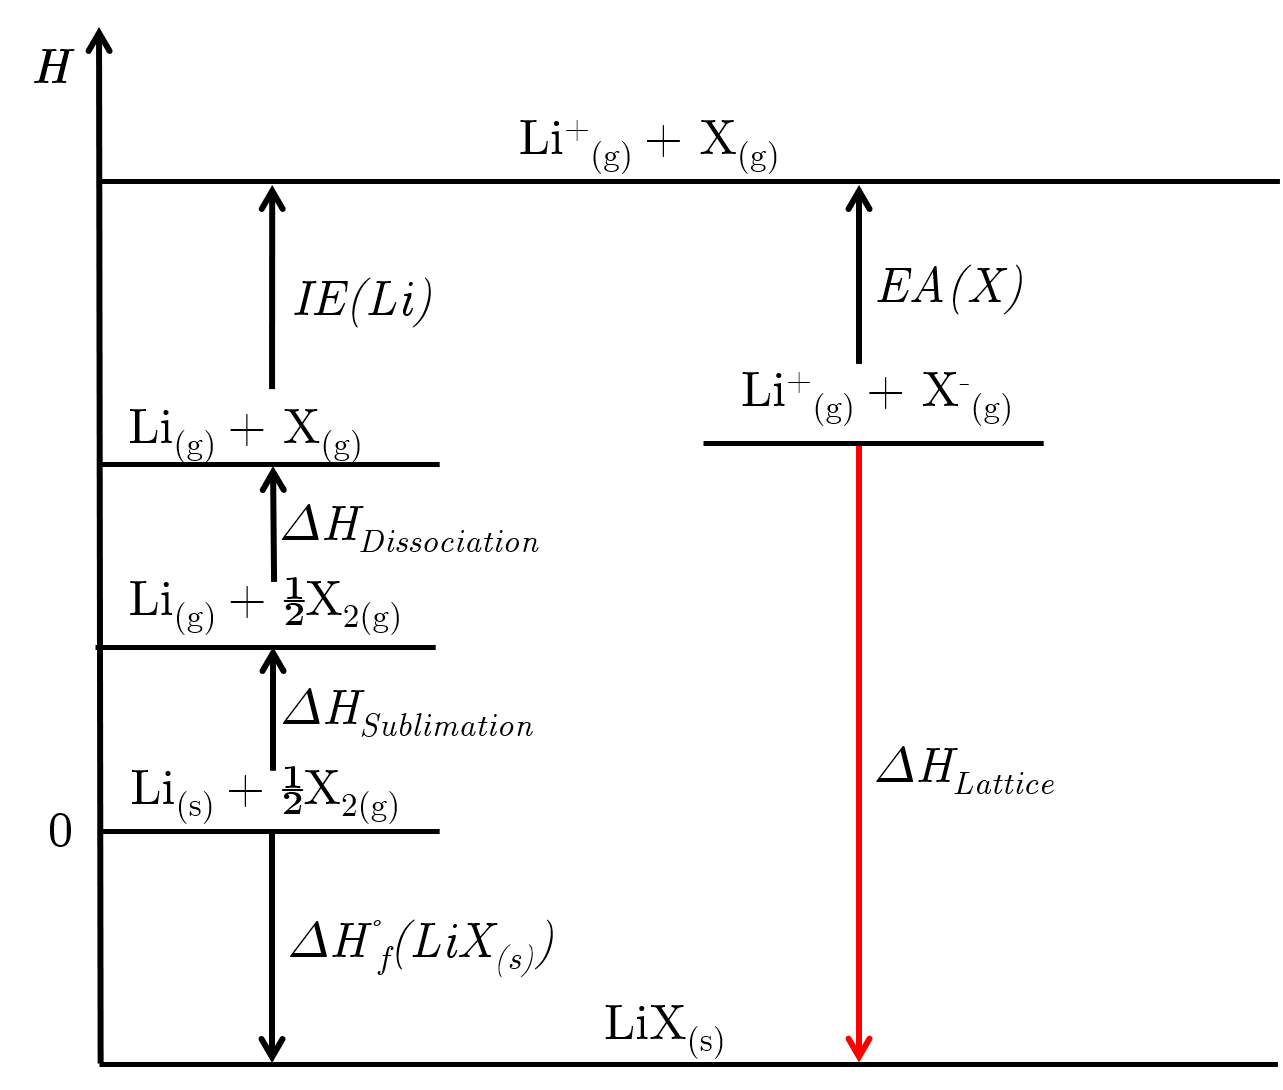
\includegraphics[width=0.8\textwidth]{Figures/Born_Haber.eps}
	\caption{An overview of the Born-Haber cycle, as used to calculate lattice enthalpy for a lithium halide (LiX) salt.}
	\label{fig:Born_Haber}
\end{figure}
%
The only true experimental lattice energies, which are used for comparison here, are those indirectly calculated via the Born-Haber cycle~\cite{book:CRC,Jenkins2005,ladd1959calculation} (see Fig~\ref{fig:Born_Haber}). The Born-Haber cycle (see Fig.~\ref{fig:Born_Haber}) utilizes Hess's law to calculate the lattice \textit{enthalpy} ($\Delta H^{\circ}_{L}$) in a roundabout way. The lattice enthalpy for any LiX salt at standard pressure and temperature ($\SI{298.15}{\kelvin}$) is calculated as
\begin{align}
\Delta H^{\circ}_{L} = \Delta H^{\circ}_{f} (\text{LiX}_{(s)}) - \Delta H_{f}^{\circ} (\text{Li}_{(g)}) - \Delta H^{\circ}_{f} (\text{X}_{(g)}) - E_{IE} (\text{Li}_{(g)}) - E_{EA} (\text{X}_{(g)})
\end{align}
where $\Delta H^{\circ}_{f} (\text{LiX}_{(s)})$ is the standard enthalpy of formation for the LiX salt; $\Delta H_{f}^{\circ} (\text{Li}_{(g)})$ is the standard enthalpy of formation of gaseous lithium (equal to the enthalpy of sublimation); $\Delta H^{\circ}_{f} (\text{X}_{(g)})$ is the enthalpy of formation for the halide atom (equal to the dissociation enthalpy); $E_{IE} (\text{Li})$ is the lithium first ionization energy; and $E_{EA} (\text{X})$ is the electron affinity of the halide, defined as the change in energy associated with the addition of a single electron. Summation of all of these quantities results in the lattice enthalpy, which for lithium halides can be separated into the following contributions (see Fig.~\ref{fig:Lattice_Energy})
%
\begin{figure}
	\centering
	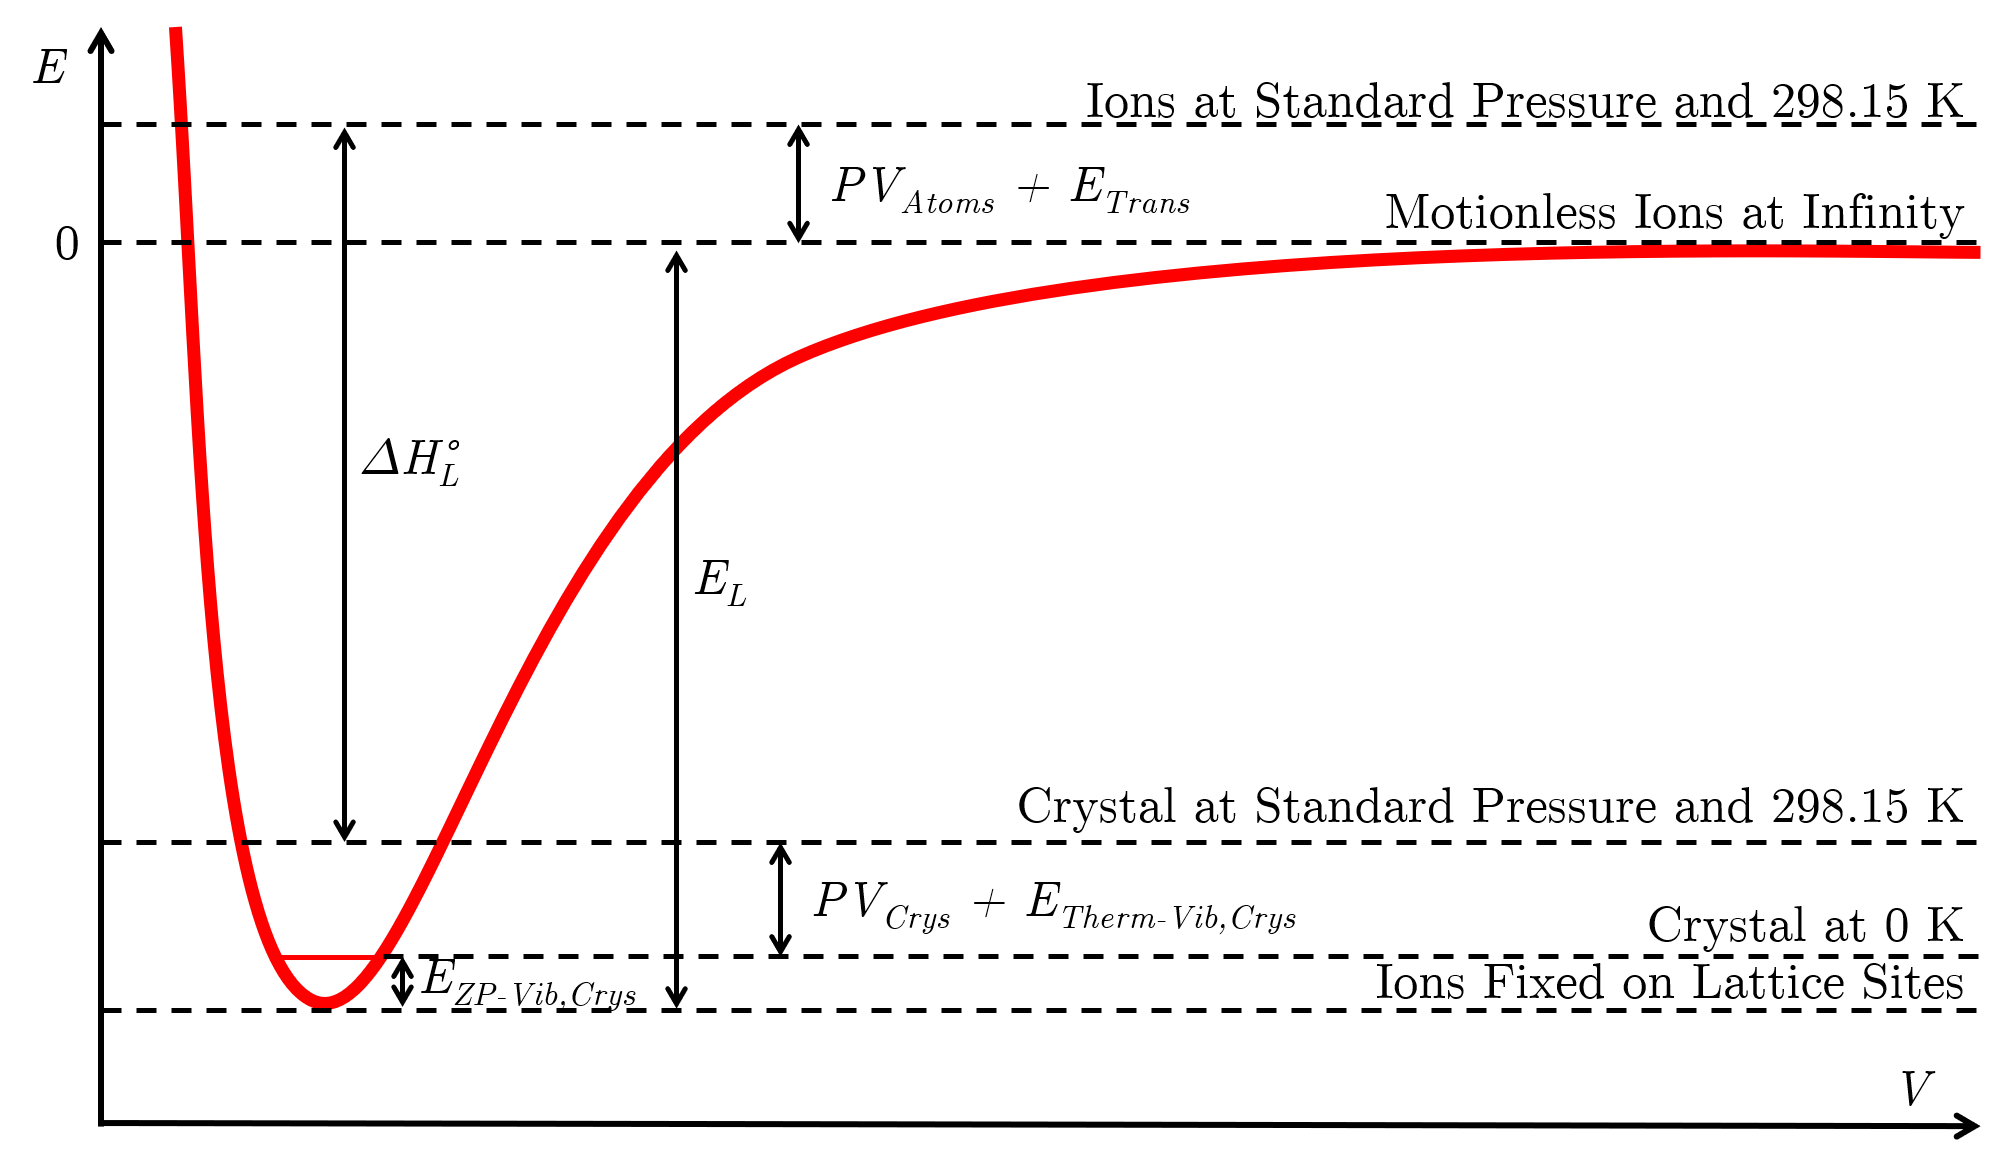
\includegraphics[width=\textwidth]{Figures/Lattice_Energy.eps}
	\caption{A diagram illustrating the thermodynamic terms associated with the calculation of lattice energies for non-molecular crystals.}
	\label{fig:Lattice_Energy}
\end{figure}
%
\begin{align}
\Delta H^{\circ}_{L} &= H^{\circ}(\text{LiX}) - H^{\circ} (\text{Li}^{+} + \text{X}^{-})\\
&= \big( U_{Crys} + E_{ZP} + E_{Vib} + PV_{Crystal} \big) - \big( U_{Ions} + E_{Trans} + PV_{Ions} \big).
\end{align}
Here we have broken up the enthalpy of the crystal into the internal potential energy $U_{Crys}$, the zero point vibrational energy $E_{ZP}$, the thermal contribution to vibrational energy $E_{Vib}$, and a $PV_{Crystal}$ term. The enthalpy of the ions is similarly broken down into an internal potential energy term $U_{Ions}$, the thermal translation energy of the ions $E_{Trans}$, and a $PV_{Ions}$ term. Note that there is no rotational energy for a system of monatomic ions. The definition of lattice energy used here is \mbox{$E_{L} \equiv U_{Crys} - U_{Ions}$}, hence
\begin{align}
\Delta H^{\circ}_{L} = E_{L} + E_{ZP} + E_{Vib} + PV_{Crystal} - E_{Trans} - PV_{Ions}.
\end{align}
No approximations have been made up to this point. From the lattice enthalpy, the typical approximate method~\cite{book:CRC,Jenkins2005} used to calculate the lattice \textit{energy} of an arbitrary non-molecular salt of type $M_{a}X_{b}$ is as follows. Note that we have defined lattice energy as the difference in the potential energy between ions at infinite separation and the crystal with all ions frozen at their equilibrium positions, without vibrational zero-point energy ($E_{ZP}$).

To begin with, one typically neglects the $PV_{Crystal}$ term of the salt enthalpy. This is justified since $PV_{Crystal}$ is typically far below the uncertainty threshold at ambient pressure. Next, the $PV_{Ions}$ term is approximated as a high-temperature ideal gas
\begin{align}
PV_{Ions} \approx  n R T,
\label{eq:PV_Ions}
\end{align}
where $n = a + b$ is the moles of (ideal) gas per mole of crystal ($2$ for a lithium halide salt). It should be noted that the assumption of ideality may seem poor in this case considering the long-range electrostatic forces between gaseous ions. However, notice that in the Born-Haber cycle the thermodynamic state of gaseous ions are never directly measured. Instead, the $PV$ measurement of gases is made only for gaseous atomic and molecular species. Furthermore, introducing a more accurate equation of state for the gas is nontrivial and unique for each gaseous species. Next, the ion translational energy $E_{Trans}$ is approximated from the equipartition theorem as~\cite{Jenkins2005}
\begin{align}
E_{Trans} \approx  \frac{3}{2} n R T = \left[ a \left( \frac { 3 }{ 2 } \right) + b \left( \frac{ 3 } { 2 } \right) \right] R T.
\label{eq:E_Trans}
\end{align}
All that remains is the vibrational terms of the crystal $E_{Vib} + E_{ZP}$. An approximation to the vibrational energy is derived from either the Debye or Einstein models for a crystal in the high temperature regime, where 
\begin{align}
E_{Vib} + E_{ZP} \approx  3 n R T = \left( 3 a  + 3 b \right) R T.
\label{eq:E_Vib}.
\end{align} 
It is expected that light salts such as LiF do not exist in the high temperature vibrational regime under ambient conditions, so this approximation overshoots the vibrational energy of such species. In addition, the classical approximation only implicitly includes the zero-point vibrational energy, which is species and structure dependent but not expected to be greater than approximately $\SI{10}{\kilo\joule\per\mole}$ for ionic salts.~\cite{froyen1984} Overall, the typical method used to calculate the lattice energy of non-molecular salts through the Born-Haber cycle is
\begin{align}
E_{L} =\Delta H - \left[ a \left( \frac { 3 } { 2 } - 2 \right) + b \left( \frac { 3 } { 2 } - 2 \right) \right] R T.
\end{align}
This method relies on a range of experimental data with a range of uncertainties and potential systematic errors, such as lattice defects in the crystalline phase and the assumption of ideal gas. In addition, the approximations used in calculating $E_{L}$ from $\Delta E$ add further uncertainty to the experimental lattice energies. It appears that no proper error analysis has been done for lithium halide lattice energies calculated via the Born-Haber cycle, and no uncertainties are reported.~\cite{book:CRC}

In light of the above situation, we decided to improve the experimental lattice energy calculations for lithium halides by delving back into the original sources for the thermochemical properties needed. It is possible to derive a more accurate lattice energy for the lithium halides from already existing thermodynamic data, as long as the vibrational zero-point energy is known. 

Measurements of the formation enthalpies for LiF and LiCl crystals have been made down to $\SI{100}{\kelvin}$ with extrapolations to $\SI{0}{\kelvin}$.~\cite{chase1998nist} Uncertainties in these measurements are reported. From this, an important reported thermodynamic quantity is derived:
\begin{align}
H^{\circ} (\text{LiX}) - H (\text{LiX}, \SI{0}{\kelvin}) = E_{vib}(\text{LiX}) + PV (\text{LiX},\SI{298}{\kelvin}) - PV (\text{LiX},\SI{0}{\kelvin}) \approx E_{vib}(\text{LiX})
\end{align}
the approximation here is almost exact at ambient pressure, as the change in volume of a crystal between $\SI{0}{\kelvin}$ and $\SI{298}{\kelvin}$ is extremely small. Similar measurements have been made for the formation enthalpies of $Li_{(g)}$ and all the atomic halides in their gas phase,~\cite{chase1998nist,cox1984codata} yielding
\begin{align}
H^{\circ} (\text{Li}_{(g)}) - H (\text{Li}_{(g)}, \SI{0}{\kelvin}) &= E_{Trans}(\text{Li}_{(g)}) + PV (\text{Li}_{(g)},\SI{298}{\kelvin}) - PV (\text{Li}_{(g)},\SI{0}{\kelvin})\\ &= E_{Trans}(\text{Li}_{(g)}) + PV (\text{Li}_{(g)},\SI{298}{\kelvin})
\end{align}
as well as the equivalent measurement for the halide. This provides all the necessary data required to calculate more accurate lattice energies, except for the vibrational zero point energy.

There are no reported experimental vibrational zero point energies available for lithium halide crystals, so we calculated them via CRYSTAL17's harmonic vibration module~\cite{Crystal17,pascale2004calculation,Crystal17Manual} using a $4\times4\times4$ supercell of each lithium halide in the rocksalt crystal structure and the PBE exchange-correlation (XC) functional. All DFT vibrational analysis calculations were performed using D3(BJ) dispersion correction.~\cite{Grimme2010,grimme2016dispersion,Becke2007,Grimme2011} We also tested three different XC functionals (PBE,~\cite{Perdew1996} PW1PW,~\cite{PW1PW} and B3LYP\cite{becke1988,lee1988,Becke1993}, but the resulting zero-point energies were consistent to within $\SI{0.5}{\kilo\joule\per\mole}$. We also tested supercells from $1\times1\times1$ to $4\times4\times4$ with PBE, and found that the calculated zero-point vibrational energy shifted less than $\SI{0.1}{\kilo\joule\per\mole}$ between $3\times3\times3$ and $4\times4\times4$ supercells for calculations of each lithium halide salt. Therefore, we consider our calculations sufficiently converged.

Putting all of these data points together results in the new lattice energies reported in table.~\ref{tab:Lattice_Energies}
%
\begin{table}
	\begin{tabular}{l|lllll}
		& LiF             & LiCl           & LiBr           & LiI            & NaCl           \\ \hline
		Approximate $E_{L}$~\cite{book:CRC} & 1049            & 864            & 820            & 764            & 790            \\
		Recalculated $E_{L}$                & 1054.2$\pm 1.3$ & 865.4$\pm 1.5$ & 821.3$\pm 1.5$ & 764.5$\pm 1.3$ & 791.0$\pm 0.8$
	\end{tabular}
\caption{\label{tab:Lattice_Energies} Approximate and updated experimental lattice energies (calculated via the Born-Haber cycle) for the lithium halides and NaCl, including uncertainties.}
\end{table}


%%% TO DO: Mention LiBr and LiI technique, summary of Data points and references with uncertainties




	The first correction one might make is for finite pressure. Thermodynamic measurements are typically reported at $\SI{1}{\bar}$, a pressure modification which slightly raises the potential energy of the crystal and has a negligible affect on the potential energy of ions. We have calculated the energy correction of lithium halide crystals (through geometry optimization including an external stress of $\SI{1}{\bar}$) to be on the order of $\SI{0.01}{\kilo\joule\per\mole}$ for LiF and $\SI{1}{\kilo\joule\per\mole}$ for LiI, which has a lower bulk modulus. Since most experimental data is unavailable at $\SI{0}{\bar}$, we are forced to make the approximation that
\begin{align}
E_{L} \approx E_{Fixed,Crys}^{\circ} (\SI{0}{\kelvin}) - E_{Ions}^{\circ} (\SI{0}{\kelvin}).
\end{align}


The next correction is for the vibrational zero-point energy of the crystal ($E^{\circ}_{ZP-Vib,Crys}$). For simple non-molecular crystals like the lithium halides,
\begin{align}
E_{Fixed,Crys}^{\circ} (\SI{0}{\kelvin}) = E_{Crys}^{\circ} (\SI{0}{\kelvin}) - E^{\circ}_{ZP-Vib,Crys}
\end{align}
where $E^{\circ}_{Crys} (\SI{0}{\kelvin})$ is the true equilibrium energy of a crystal at $\SI{0}{\kelvin}$, accounting for the crystal's vibrational zero-point energy. Since experimental measurements are typically done at room temperature, one must also correct for thermal effects. As there are no rotational degrees of freedom for non-molecular crystals, and other partitions of energy --- such as electronic and nuclear energy --- are unaffected by thermal fluctuations at $\SI{298.15}{\kelvin}$,
\begin{align}
E^{\circ}_{Crys} (\SI{0}{\kelvin}) = E^{\circ}_{Crys} (\SI{298.15}{\kelvin}) - E^{\circ}_{Therm-Vib,Crys} (\SI{298.15}{\kelvin}).
\end{align}
Where $E^{\circ}_{Therm-Vib,Crys} (\SI{298.15}{\kelvin})$ is the thermal contribution to the crystal's vibrational energy at $\SI{298.15}{\kelvin}$. Similarly for the spherically symmetric ions,
\begin{align}
E^{\circ}_{\text{Ions}}(\SI{0}{\kelvin}) = E^{\circ}_{Ions}(\SI{298.15}{\kelvin}) - E^{\circ}_{Trans} (\SI{298.15}{\kelvin})
\end{align}
where $E^{\circ}_{Trans} (\SI{298.15}{\kelvin})$ refers to the translational energy of the ions at $\SI{298.15}{\kelvin}$. With these corrections, Eq.~\ref{eq:Lattice_Energy_Def} becomes
\begin{equation}
\begin{split}
\label{eq:Lattice_Energy2}
E_{L} &= E^{\circ}_{Crys} (\SI{298.15}{\kelvin}) - E^{\circ}_{Therm-Vib,Crys} (\SI{298.15}{\kelvin}) - E^{\circ}_{ZP-Vib,Crys} (\SI{298.15}{\kelvin})\\ &- E^{\circ}_{Ions}(\SI{298.15}{\kelvin}) + E^{\circ}_{Trans}(\SI{298.15}{\kelvin}).
\end{split}
\end{equation}
The terms $E^{\circ}_{Crys} (\SI{298.15}{\kelvin})$ and $E^{\circ}_{Ions}(\SI{298.15}{\kelvin})$ are potential energies which are not easily measured directly, but can instead be derived from enthalpy differences. If one adds and subtracts off pressure-volume terms for both the ions and the crystal








 
\begin{acknowledgments}
The financial support of the Natural Science and Engineering Research Council of Canada is gratefully acknowledged. This research has been enabled by the use of WestGrid and Compute Canada computing resources, which are funded in part by the Canada Foundation for Innovation, Alberta Innovation and Science, BC Advanced Education, and the participating research institutions. WestGrid and Compute Canada equipment is provided by IBM, Hewlett Packard and SGI.
\end{acknowledgments}

\clearpage
%\section*{References}
\bibliography{references}

\end{document}
